\cotefile{57}
\scanpage{133}
% lines 1–5
\uline{Théorème}$^{\ast}$ Soit \deleted{$\unsure{Y'\!-\!X'|Y'\leftarrow X'|X'\to X''}$} \inserted{$f:X\unsure{-|\to}Y$} un morphisme \uline{surjectif} de préschémas propres sur un corps $k$. Alors le noyau $\underline{\underline{N}}$ de $\underline{\underline{\mathrm{Pic}}}_{\deleted{X}Y/k}-\underline{\underline{\mathrm{Pic}}}_{X/k}$ est \margin{?}\deleted{contenu} un sous-groupe d'un \uline{groupe} \uline{affine} $G$ sur $k$.

% lines 6–8
\unsure{Donc}

\uline{Corollaire} Si $\underline{\mathrm{Pic}}_{Y/k}$ et $\underline{\mathrm{Pic}}_{X/k}$ existent, le noyau de $\underline{\mathrm{Pic}}_{Y/k}-\underline{\mathrm{Pic}}_{X/k}$ est un groupe alg. affine.

% lines 9–14
\uline{Corollaire} Sous les conditions précédentes, \unsure{on} $\text{Nér Sév}_{0}(Y/\unsure{k})-\text{Nér Sév}_{0}(X/k)$ est \uline{injectif}, et \deleted{\unsure{Q}} si $A$ et $B$ sont les ``parties abéliennes'' de $\underline{\mathrm{Pic}}_{Y/k}$ et $\underline{\mathrm{Pic}}_{X/k}$ [définies si $k$ est parfait] alors $A\to B$ a un noyau fini.

% lines 15–19
\uline{Dém} \deleted{$\underline{\mathrm{Pic}}_{X}-\underline{\mathrm{Pic}}_{Y}$} On va pour simplifier admettre que tous les $\underline{\mathrm{Pic}}$ envisagés sont représentables. \inserted{a) On peut supposer $k$ \uline{alg. clos} (\unsure{Sert à rien|Suffira|ou non} ?)} b) On aura un diagramme de \uuline{schémas} sur $k$
\diagram{\begin{tikzcd}[ampersand replacement=\&]
\underline{\mathrm{Pic}}_{X/k}\arrow[d,dash] \& \underline{\mathrm{Pic}}_{Y/\unsure{k}}\arrow[l]\arrow[d,"\text{\uline{affine}}"] \& {} \\
\underline{\mathrm{Pic}}_{X_{\mathrm{réd}}} \& \underline{\mathrm{Pic}}_{Y_{\mathrm{red}}}\arrow[l,"?"'] \& {}
\end{tikzcd}\(\left.\vphantom{\begin{matrix}X\\X\\X\end{matrix}}\right]\text{ par \unsure{vert|vert.|dont}}\)}
% archive sheet number: 132

\scanpage{134}
% lines 1–5
\[
\underline f^{m-n}: K_{*}(\underline f^{m})\qquad K_{*}(\underline f^{n})
\]
ou $m$ et $n$ sont des entiers rationnels, $m\quad n\quad 0$, d'ou des \deleted{\unsure{en|un}}homomorphismes, notes par le meme symbole:
\[
\begin{aligned}
& K^{*}(\underline f^{n},M)\quad K^{*}(\underline f^{m},M)\\
\text{et}\qquad & H^{*}(\underline f^{n},M)\quad H^{*}(\underline f^{m},M)\qquad (m\quad n\quad 0).
\end{aligned}
\]
% lines 6–13
Comme ces homomorphismes sont transitifs, on peut passer a la limite inductive dans ces homomorphismes, et poser
\[
\begin{aligned}
C^{*}((\underline f^{\deleted{\unsure{n}}}),M)&=\lim_{n} K^{*}(\underline f^{n},M)\\
\underline H^{*}((\underline f^{\deleted{\unsure{n}}}),M)\deleted{\unsure{*}}&=H^{*}(C^{*}((\underline f),M)=\lim_{n}H^{*}(\underline f^{n},M).
\end{aligned}
\]
(N.B. dans ces notations, $(\underline f)$ designe en fait l'ideal engendre dans $A$ par les $f_i$; on verra en effet ulterieurement que les objets introduits, \deleted{\unsure{ne dependent}} du moins $H^{*}((\underline f),M)$, ne depend aue de cet ideal, et meme seulement de la topologie $\underline m$-adique \deleted{\unsure{a}}qu'il definit, et non des $f_i$ eux-memes\unsure{.} 

% lines 14–22
Bien entendu, $C^{*}((\underline f),M)$ est un foncteur \deleted{exact} ($A$-lineaire exact) en $M$ et $H^{*}((\underline f),M)$ est un foncteur cohomologique en $M$.

Soit $\underline f$ comme ci-dessus, \deleted{\unsure{soit}} considere comme element du dual de $A^{n}$, soit $\underline g=(g_i)_{1\quad i\quad n}$ un element de $A^{n}$ lui-meme, on sait qu'on a alor\deleted{\unsure{x}}s, en designant par $e_{\underline g}$ l'operation de multiplication exterieure par $\underline g$ dans $A^{n}$, la \uline{formule} \uline{d'homotopie}
\[
i_{\underline f}e_{\underline g}+\unsure{e}_{\underline g}i_{\underline f}=\langle\underline g,\underline f\rangle\mathrm{id}.
\]
dans $A^{n}$, qui peut aussi s'ecrire, dans le complexe $K_{*}(\underline f)$, comme
\[
d\unsure{e}_{\underline g}+e_{\underline g}d=\underline g,\underline f\ \mathrm{id}.
\]
% lines 23–28
On en conclut la

\uline{Proposition 1}. Supposons que l'ideal $(\underline f)$ engendre par les $f_i$ soit $A$. \unsure{Alors} le complexe $K_{*}(\underline f)$ est homotopiquement equivalent a zero, et il en est \unsure{par} suite dememe des complexes $\unsure{K|H}_{*}(\underline f,M)$ et $K^{*}(\underline f,M)$ quels que soit $M$.
% slanted
\margin{\handwritten{\unsure{Autre|Plus|Ajouter un}, corollaire: les $f_i$ annulent les $H_{*}(\underline f,M)$, $H^{\cdot}(f,M)$}}

\uline{Corollaire} S'il en est ainsi, on a $H^{*}(\underline f,M)=0$ et $H^{*}((\underline f),M)=0$ pour \unsure{tout} $A$-module $M$.

% lines 29–38
Dans la description de $K^{*}(\underline f,M)$, il faut aussi ajouter \unsure{l'interpretation} des elements de degre $p$ de ce complexe comme des fonctions alternees de $p$ indices variables entre $1$ et $n$; la formule du cobord est alors formellement celle d'un cobord en cohomologie de Cech.

2. \uline{Cohomologie de Cech d'un recouvrement ouvert}.

Soient $X$ un preschema, $A=\mathrm{I}\ (X,\underline{\mathrm O}_{X})$, $\underline f=(f_i)_{1\quad i\quad n}$ un systeme de $n$ \unsure{elements} de $A$, $U_i=X_{f_i}$, $U=\quad U_i$, $\underline U$ le recouvrement de $U$ par les $U_i$. Soit $F$ un faisceau quasi-coherent sur $X$, posons
\[
M=\mathrm{I}\ (X,F)
\]
(N.B. les notations precedentes devraient etre deployees de meme !)
% archive sheet number: 133

\scanpage{135}
% lines 1–3
\deleted{d) Considérons alors la factorisation de Stein.
\[
f\qquad X\longrightarrow Y'\unsure{-|\to}Y
\]}
\unsure{Cela|Ceci} nous ramène au cas où $Y$ est \uline{réduit}.

% lines 4–12
c) \unsure{Prenons} la factorisation de Stein
\[
X-Y'-Y\deleted{\unsure{'}}
\]
où $Y'-Y\deleted{\unsure{'}}$ est fini surjectif, donc un épimorphisme fini factorisable en produit d'épimorphismes stricts. Par ``Seshadri'', $\underline{\mathrm{Pic}}_{Y}-\underline{\mathrm{Pic}}_{Y'}$ est affine. On est ramené \deleted{à prouver que $\underline{\mathrm{Pic}}_{Y'}-\underline{\mathrm{Pic}}_X$ l'est, \unsure{ou}} ce qui nous ramène au cas $f_{*}(\underline O_X)\simeq \underline O_Y$

% lines 13–15
d) Mais dans ce cas on sait aussitôt que $\underline{\mathrm{Pic}}_X-\underline{\mathrm{Pic}}_Y$ est un \unsure{mono}, donc \deleted{\unsure{un noyau est}} une immersion fermée, donc affine

% slanted
\margin{Attention au fait que $\underline{\mathrm{Pic}}_X$ et $\underline{\mathrm{Pic}}_Y$ ne sont pas de type fini sur $k$, \unsure{on aura d'inf|on aura d'of} donc pas \unsure{néc$^{t}$} affine [ex. $\mathbb Z\to G$, $G=\unsure{\mathrm G_m|G_a|\mathrm{Grass}}$ ou \unsure{courbes|$G_a$} ou VA]}

% lines 16–18
NB. On s'est servi de l'existence des $\underline{\mathrm{Pic}}_Z$ pour $Z=Y_{\mathrm{réd}}$, $X_{\mathrm{réd}}$, et pour les préschémas finis sur $Y_{\mathrm{réd}}$ ; \deleted{\unsure{Est}} on peut sans doute s'en passer \unsure{\textemdash]|(?)\textnormal{]}}.
% archive sheet number: 134

\scanpage{136}
% lines 1–10
La codim coh de $M$ sur $B$ est celle de $\overline M$ sur $\overline B$. On en déduit: sous les conditions de cor.2, la codim. coh. de $M$ sur $B$ est identique à celle de $\overline M$ sur $\overline A$ (l'énoncer en corollaire; je m'aperçois que le cor.3 précédent devrait s'énoncer ainsi, avec : par conséquent $\dim_B M\quad\dim A$). On dit qu'un module de type fini sur un anneau local noethérien est Coh Mac si sa dim est égale à sa codim coh d'où un certain nombre de conséquences du lemme (qu'on peut donner en corollaires): Coh. Mac. est invariant par complétion, par changement fini d'anneau, enfin sous les conditions du cor.2 précédent \deleted{\unsure{on}}, $M$ est Coh Mac sur $B$ si et seulement si $\overline M$ l'est sur $\overline A$. Enfin rappeler que si l'anneau local est régulier, Cohen Mac sur lui signifie libre.

% lines 11–15
En fait, il faudrait sans doute un lemme spécial pour les Coh. Mac, en tous points parallèle (avec ses corollaires) au lemme sur la cocodim, mais contenant en plus le coup du régulier, et peut-être (pour avoir tout ensemble) l'équidimensionnalité. Pour l'instant, il n'était guère question de platitude dans ce numéro, mais:

% lines 16–19
\uline{Proposition} Soient $A\quad B$, \deleted{\unsure{$M$ comme|$M$ comme par le passé}} un hom local d'anneaux locaux noethériens, $M$ un $B$-module de type fini. Pour que $M$ soit $A$-plat, il faut et il suffit que $\overline M$ (le complété du $B$-module $M$ pour sa topologie naturelle) soit plat sur $\overline A$.

% lines 20–24
Il faut évidemment noter que $\overline M$ (qui n'est pas en général le complété $\underline m$-adique de $A$, puisqu'onne fait pas d'hypothèse quasi-finie) est cependant un module sur $\overline A$. - Démonstration: On applique le critère de prop.13, en notant que $\operatorname{Tor}^{A}_{1}(\underline k,M)$ est un $B$-module de type fini, et que son complété est $\operatorname{Tor}^{\overline A}_{1}(\underline k,\overline M)$.

% lines 25–28
\uline{Corollaire} 1 Supposons de plus $M$ qu f sur $A$. Alors $M$ plat sur $A$ équivaut à $\overline M$ libre sur $\overline A$.

\uline{Corollaire} 2 Supposons $M$ comme dans le cor.1 et $A$-plat, $\ne 0$. Alors
\[
\dim_B M=\dim A\qquad \operatorname{cocodim}_{B}M=\operatorname{cocodim}_{\overline{\unsure{A|B}}}\overline A
\]
% lines 29–33
En effet, dim et cocodim sont invariants par complétion, d'autre part par changement \unsure{raisonnablo|raisonnable} d'anneau, ce qui nous ramène d'abord au cas où $B$ lui-même\deleted{\unsure{s}} est qu f sur $A$, puis par complétion au cas où $A$ et $B$ complets (donc $B$ fini sur $A$) puis encore au\deleted{\unsure{x cas| cas}} $A=B$, enfin on note que la dim - cocodim d'une somme directe est le sup resp. inf des dim \unsure{re|res}
% archive sheet number: 135

\scanpage{138}
% lines 1–2
Soit $f:X\unsure{-|\to} S$ un morphisme se factorisant en $X\overset{\varphi}{-}\Sigma\overset{\psi}{-}S$, avec $\psi$ fini, et $\varphi$ tel que $\underline O_\Sigma\overset{\sim}{\longrightarrow}\varphi_{*}(\underline O_X)$.

% lines 3–8
1) Alors \unsure{on a}
\[
\unsure{\cdot|0}\to\mathrm{Pic}(\Sigma)-\mathrm{Pic}(X)-\mathrm{Pic}'(X/S)
\]
[suite exacte provenant de la suite spectrale de Leray].

\deleted{\unsure{et}} \uline{Si} $X/\Sigma$ admet une section, le dernier hom est un isom, i.e. dans ce cas
\[
\mathrm{Pic}'(X/S)\simeq\mathrm{Pic}(\deleted{\Sigma}X)/\mathrm{Pic}(\deleted{\unsure{X|\Sigma}}\Sigma)
\]
% lines 9–16
Ce dernier fait se voit ainsi: \deleted{Pour} Soit $g:\Sigma\longrightarrow X$ une section de $X/\Sigma$ ; alors \inserted{ii) \unsure{puis|pour}} \deleted{\unsure{tout}} \unsure{1|Les} Module inversible $g$-rigidifié sur $X$ n'a pas d'aut. non trivial, \inserted{iii)} tout Module inversible $\underline L$ sur $X$ est \deleted{\unsure{de isom|de façon}} $\mathrm{Pic}'(X/S)$ \uline{équivalent} à \deleted{l'image} un Module inversible $g$-rigidifié \inserted{[savoir $\underline L\otimes\varphi^{*}(g^{*}(\underline L))$]} [déterminé à isom unique près].

[On utilise le fait que $\mathrm{Pic}'(\Sigma/S)=0$].

% last line
On suppose pour la suite \deleted{\unsure{f}} que, quel \unsure{de|est} que soit
% archive sheet number: 137

\scanpage{139}
% lower half, upright
\diagram{\begin{tikzcd}[ampersand replacement=\&,row sep=small]
{} \& S\\
\Sigma\arrow[ur] \& {}\\
{} \& X\arrow[ul]\arrow[uu]
\end{tikzcd}}
% lower block written upside down
\deleted{\diagram{\begin{tikzcd}[ampersand replacement=\&]
X\arrow[d,"f"'] \&[-1.4em] \underset{i}{\supset} \&[-1.4em] Z\ \text{fermé}\arrow[dll,"\varphi"]\\
S \& {} \& {}
\end{tikzcd}}
Supposons

(i) $Z$ fini sur $S$

(ii) $f_{*}\unsure{(\underline O_X)|\underline O_X)}\overset{\sim}{\longrightarrow}\varphi_{*}(\underline O_S)$

Alors (i) Tout Module inversible sur $X$ est $\mathrm{Pic}'(X/S)$-équivalent\unsure{,} \unsure{un|à un} Module}
% archive sheet number: 138

\scanpage{140}
% lines 1–6
2) Soit $S'\unsure{-|\to}S$ fid. plat et qu. cpt. Alors

(i) $\mathrm{Pic}'(X/S)-\mathrm{Pic}'(X'/S')$ est injectif. (ii) Si $X/\Sigma$ a \deleted{\unsure{loc.}} une section, \deleted{\unsure{sur}} localement sur $S$, alors
\[
\mathrm{Pic}'(X/S)\to\mathrm{Pic}'(X'/S')\rightrightarrows\mathrm{Pic}'(X''/S'')
\]
est exact.
% slanted
\margin{Généraliser à des ``quasi-sections'' du type \unsure{$N^{*}$|$N^{\circ}$} dès l'abord \textemdash}

% lines 7–10
On peut dans (i) partir d'un $\underline L$ inv. sur $X$. \inserted{En vertu de 1),} L'hyp. signifie que $\underline L'$ provient de $\Sigma'$. Or $\Sigma'$ est fid plat qu. cpt sur $\Sigma$. On sait qu'alors \deleted{\unsure{le}} $L$ provient de $\Sigma$.

% lines 11–15
Pour (ii), \inserted{\unsure{grâce à|après|qui est} (i),} la question est locale sur $S$, on peut donc supposer que $X$ a une section sur $\Sigma$. Alors on utilise la théorie de descente comme dans le raisonnement connu.

% lines 16–20
\uline{Corollaire} \deleted{\unsure{1}} Sous les conditions précédentes, $\mathrm{Pic}'(X/S)\to\mathrm{Pic}^{*}(X/S)$ est injectif, et \unsure{même|est} bijectif si $X/\Sigma$ \deleted{\unsure{loc une}} a une section loc. sur $S$ ; Si $X/\Sigma$ a \unsure{\textnormal{même}} une section, on a un isom
\[
\mathrm{Pic}(X/S)\simeq\mathrm{Pic}(X)/\mathrm{Pic}(\Sigma)
\]
% archive sheet number: 139

\scanpage{141}
Picard des schémas \unsure{en|ou} courbes
% archive sheet number: 140

\scanpage{142}
% lines 1–5
$f:X\to S$ projectif et lisse, fibres géom connexes de dim 1.

$U=X-Y$, \inserted{$Y$ sous-schéma fermé de $X$ \uline{étale} sur $S$} \deleted{\unsure{$Y$}} [\inserted{p. ex. $Y=$} $\coprod_{i\in I}g_i(S)$, les $g_i$ des sections telles que les $g_i(S)$ deux à deux disjoints]

$f_U:U-S$

$n$ premier aux car. résiduelles \inserted{de $S$}. On trouve
\[
E^{pq}_{2}=H^p(S,\underbrace{R^q_{!}f_U(\mu_n)}_{\substack{0\ \text{sauf si}\\q=1,2}})\Longrightarrow H^{*}_{\mathrm{prop}}(\deleted{\unsure{X}}U,\mu_n)
\]
% lines 6–9
\[
R^q_{!}f_U(\mu_n)=
\begin{cases}
0 & \text{si }q\deleted{\ne}\inserted{\notin}\{1,2\\
{}_{n}E & \text{si }q=1\qquad\text{(cf plus bas \inserted{déf. de $E$})}\\
(Z/nZ)_S & \text{si }q=2
\end{cases}
\]
\figure{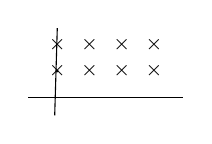
\begin{tikzpicture}[x=.41cm,y=.33cm]
\draw (-.9,0)--(3.9,0); \draw (-.08,-.7)--(0,2.65);
\foreach \x in {0,1,2,3}{\foreach \y in {1,2}{\node at (\x,\y) {\scriptsize $\times$};}}
\fill (0,1) circle (.05);
\end{tikzpicture}}
\diagram{\begin{tikzcd}[ampersand replacement=\&,row sep=small]
E_2^{02}\arrow[r]\arrow[d,equal] \& E_2^{2,1}\arrow[d,equal]\\
H^0(S,Z/nZ) \& H^2(S,{}_{n}E)
\end{tikzcd}}

% lines 10–14
On trouve un élément canonique
\[
\xi_n\in H^2(S,{}_{n}E)
\]
Si $n=l^{\unsure{\nu|v}}$ ($\nu$ variable), $l$ premier distinct des car. rés. sur $S$, on trouve
\[
\boxed{\xi(l)\in H^2(S,T_l(E))}
\]
Cet \uline{élément est nul si} $U$ a \uline{une section sur} $S$.

% lines 15–18
$E$ est un schéma en groupes lisse sur $S$, \deleted{\unsure{tel}} \inserted{à fibres connexes,} extension de $J=\underline{\mathrm{Pic}}^{0}_{X/S}$ par $T=G_m^{I}/\underset{\longrightarrow\,\text{diagonale}}{G_m}$,
\diagram{\begin{tikzcd}[ampersand replacement=\&,row sep=small]
0\arrow[r] \& T\arrow[r]\arrow[d,equal] \& E\arrow[r] \& J\arrow[r] \& 0\\
{} \& G_{m_S}^{I}/G_{m_S} \& {} \& {} \& {}
\end{tikzcd}}
% archive sheet number: 141

\scanpage{143}
% letterhead
INSTITUT\\
DES HAUTES ÉTUDES SCIENTIFIQUES\\
91 - BURES-SUR-YVETTE\\
928-48-53\\

Massy November 21, 1966\\

Dear Mr Benjamin,\\

I got the front matter for the book ``Huit exposés ... '', which I am now sending back to you with two minor corrections. A more serious matter - and this is why I am adressing this letter to you rather than to Miss Ball \margin{\handwritten{\unsure{?}}} - is the interrogation mark on page three concerning the mention ``Copyright 1966 by W.A. Benjamin, Inc ''. In your letter of july 8 1966, you stated that the copyright would remain with Mr Bourbaki, and I have been assuming till now that the book was being published under this proviso. If you should have changed your mind about it, I will have to check with Bourbaki if it is all right with him, which (whatever his decision) will cause a delay of a few months more. Once th\deleted{\unsure{u|e}}is matter set straight, everything is all right with me resp. the front matter, and you can go ahead\deleted{x} with the printing. I would only like to know if you got m\deleted{\unsure{u}}y letter of November 10 proposing to include still another paper, and your opinion about this suggestion.

Sincerely yours\\
% archive sheet number: 142

\scanpage{144}
% lines 1–6
On obtient $E$ ainsi : \deleted{\unsure{collapsant|collapsons} $Y$} On définit un schéma en courbes plat $Z$ sur $S$ comme conoyau de
\diagram{\begin{tikzcd}[ampersand replacement=\&,column sep=large]
X\amalg(Y\times_S Y)\arrow[r,shift left=1.15ex,"{\mathrm{id}_X,\alpha\operatorname{pr}_1^{Y/S}}"]\arrow[r,shift right=1.15ex,"{(\mathrm{id}_X,\alpha\operatorname{pr}_2^{Y/S})}"'] \& X \& (\alpha:Y\hookrightarrow X)
\end{tikzcd}}
et on définit
\[
E=\underline{\mathrm{Pic}}^{0}_{Z/S}.
\]

% lines 7–11
\deleted{\unsure{Remarque}} Le morphisme $E\to J$ est induit par $X\xrightarrow{\varphi} Z$ en passant au $\underline{\mathrm{Pic}}^{0}_{-/S}$. Notons que nous avons un torseur canonique $P$ sous $E$,
\[
P=\underline{\mathrm{Pic}}^{1}_{Z/S}
\]
(et, d'ailleurs, un $S$-morphisme can $U\to P$).

% lines 12–19
Notons que $P$ définit un élément
\[
\boxed{\unsure{\eta|y}\in H^1(S,E)},
\]
et la relation entre $\xi_n$ et $\eta$ est
\[
\boxed{\xi_n=\delta_n(\eta)},
\]
\margin{à vérifier \unsure{......}}
où $\delta_n$ est l'opérateur cobord
\[
H^1(S,E)\unsure{-|\to}H^{\unsure{2|1}}(S;{}_{n}E)
\]
associé à la suite exacte de Kummer
\[
0\to{}_{n}E\to E\overset{n\,\mathrm{id}_E}{-}E-0.
\]
% archive sheet number: 143

\scanpage{145}
% lines 1–8
Notons que l'image de $\unsure{\eta|y}$ dans $H^1(S,J)$, par fonctorialité, n'est autre que la classe \deleted{de} $\underline{\mathrm{Pic}}^1_{X/S}$ (considéré comme torseur sous $J$). Supposons cette classe nulle (ce qui est le cas si $X/S$ admet une section). \deleted{\unsure{p. ex.}} Alors la suite exacte
\[
H^0(S,J)\longrightarrow H^1(S,T)\to H^1(S,E)\unsure{-|\to}H^1(S,J)
\]
montre que \deleted{\unsure{le}} $\eta$ est dans $\operatorname{Im}H^1(S,T)$.

% lines 9–13
Notons qu'on a d'ailleurs une suite exacte \inserted{(si $Y-S$ surjectif)}
\[
0\to G_{m_S}\to\prod_{Y/S}G_m\to T-0 \tag*{($*$)}
\]
qui donne une suite exacte \deleted{\unsure{écrite}}
\[
\unsure{0|\cdot}\to H^0(S,\underline O_S)^{\unsure{*}}\to H^0(Y,\underline O_Y)^{*}\to H^0(S,T)-\mathrm{Pic}(S)\to\mathrm{Pic}(Y)-H^1(S,T)\to\mathrm{Br}'(S)\to\mathrm{Br}'(Y),
\]

% lines 14–21
Lorsque la suite exacte ($*$) splitte, p. ex. lorsque $Y$ admet une section sur $S$, alors on trouve
\[
\deleted{H^1(S,T)=}\qquad H^1(S,T)\simeq\mathrm{Pic}(Y)/\operatorname{Im}\mathrm{Pic}(S)
\]
et lorsque $Y=\coprod_{i\in I} g_i(S)$ comme dessus, alors \deleted{\unsure{on peut}} $\mathrm{Pic}(Y)\simeq\mathrm{Pic}(S)^I$ et on trouve
\[
H^1(S,T)\simeq\mathrm{Pic}(S)^I/\underset{\longrightarrow\,\text{par diagonale}}{\operatorname{Im}}\mathrm{Pic}(\deleted{\unsure{X}}S).
\]
Si p. ex. $\mathrm{Pic}(S)=0$, on trouve $\eta=0$, à fortiori les $\xi_n$, $\xi_l$ sont nuls.
% archive sheet number: 144

\scanpage{147}
% lines 1–4
Soit $C$ une courbe complète, réduite et connexe sur $k$ \inserted{alg. clos}

On veut calculer $\mathrm{Pic}_C$
\[
\unsure{\cdot|0}\unsure{-|\to}\underline O_C^{*}-\underline{\widetilde O}_C^{*}\to\prod_P A_P^{\unsure{*}}-0\qquad P\ \text{les pts doubles}
\]
\[
\cdot\to\underbrace{G_m-\deleted{\unsure{P}}\prod_{C_i}G_m\to\prod_{P_\alpha}A_P}_{\text{\unsure{gr.|tor.|fin|tore}}}\to\mathrm{Pic}_{C/k}\to\deleted{\unsure{\mathrm{Pic}}}\prod\mathrm{Pic}_{\widetilde C_i/k}\to0
\]
\margin{$k[[t]]/t^2$}
\figure{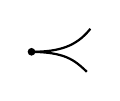
\begin{tikzpicture}[x=.65cm,y=.65cm]
\fill (0,0) circle (.075); \draw[thick] (0,0) .. controls (.55,0) and (.88,.11) .. (1.15,.45); \draw[thick] (0,0) .. controls (.65,-.01) and (.83,-.15) .. (1.08,-.39);
\end{tikzpicture}}

% lines 5–9
On trouve que l'on a \deleted{dans} $\mathrm{Pic}_{C^{0}/k}$ une partie linéaire, \deleted{et \unsure{en fait} multiplicative,} qui est isomorphe \deleted{à}
\[
G=\left(\prod_{P_\alpha}A_{P_\alpha}\right)\big/\left(\prod G_m/G_m\right)
\]
donc est de dimension égale à
\[
\dim G=\sum\mu_\alpha-c_0+1
\]
% slanted
\margin{$c_0=$ nb des comp. de $C_i$}
% lines 10–11
où $\mu_\alpha=\dim P_\alpha\inserted{=\dim_k\underline O_{\widetilde C}/\underline O_C}$ \deleted{\unsure{pour simplifier} \unsure{en} $P_\alpha$}. Posons $\mu_\alpha=1+\delta_\alpha$, \deleted{on trouve donc}

% lower cancelled block, lines 12–18
\deleted{\[
\dim G=c_1-c_0+1+\sum\delta_\alpha=b_1+\sum\delta_\alpha
\]
\deleted{\unsure{de}} où $b_1$ est le nb de cycles du schéma combinatoire de $C$.}
\margin{$c_0-c_1=1-b_1$}
\deleted{La dimension de la partie \deleted{multiplicative} \inserted{additive} de $G$ est
\[
\begin{aligned}
&\deleted{\sum_\alpha\unsure{(\nu_\alpha-1)}=\left(\sum\unsure{\nu_\alpha}\right)-c_1=2c_0-c_1=}\\
&\deleted{\sum_\alpha(\mu'_\alpha-\unsure{1})-c_0+1}\qquad\sum(\mu_\alpha-\mu'_\alpha)
\end{aligned}
\]
où $\mu'_\alpha$ est la multiplicité ``ensembliste'' de $P_\alpha$, $=$ nb de \deleted{\unsure{courbes}} \inserted{branches \unsure{formelles|simples}} passant \deleted{\unsure{e}} par $\alpha$.}
% archive sheet number: 146

\scanpage{148}
\mspage{42}
% lines 1–6
let $D_h'=\handwritten{\widetilde{\Phi}}^{-1}(D_h^{*\,\prime})$. Clearly $D_h^{*\,\prime}$ meets $D_h^{*}$ at simple intersection points only and therefore $(D_h^{*2})=(D_h^{*}D_h^{*\,\prime})$ is equal to the number of these intersection points, while each intersection point of $D_h^{*\,\prime}$ and $D_h^{*}$ corresponds to $m$ intersection points of $D_h'$ and $D_h$. Hence we have
\[
(D_h^2)=(D_hD_h')\geqq m(D_h^{*2})=2mah^2,
\]
% lines 7–11
and therefore
\[
\dim\handwritten{\big|}D_h\handwritten{\big|}\geqq mah^2-bh+\handwritten{\chi}(\overset{\handwritten{\scriptscriptstyle\sim}}{V})-1-\overset{\handwritten{\scriptscriptstyle\sim}}{p}_g,
\]
where $2b=(KD_1)$ and $\overset{\handwritten{\scriptscriptstyle\sim}}{p}_g$ is the geometric genus of $\overset{\handwritten{\scriptscriptstyle\sim}}{V}$. Combined with the equality
\[
\dim\handwritten{\big|}D_h\handwritten{\big|}=\dim\handwritten{\big|}D_h^{*}\handwritten{\big|}=ah^2-b^{*}h+\handwritten{\chi}(V*)-1,
\]
% lines 12–20
this proves that
\[
mah^2-bh\leqq ah^2-b^{*}h+\mathrm{const.},\quad\text{for all}\quad h\geqq1,
\]
where $a=\frac12(D_1^{*2})$ is positive. Consequently we obtain $m=1$. Thus the inverse image $\handwritten{\widetilde{\Phi}}^{-1}(\handwritten{\unsure{\mathfrak p|p}}*)$ of the general point $\handwritten{\mathfrak p}*$ on $V*$ consists of a single point and therefore $\handwritten{\widetilde{\Phi}}^{-1}$ has no branch curve. Hence $\handwritten{\widetilde{\Phi}}^{-1}$ is regular and single-valued except for a finite number of fundamental points. $\handwritten{\widetilde{\Phi}}$ is therefore bi-regular on $\overset{\handwritten{\scriptscriptstyle\sim}}{V}$ except for a finite number of fundamental curves.

% lines 21–22
Now these fundamental curves can be eliminated by quadratic transformations. Namely, by applying a finite number of
% archive sheet number: 147

\scanpage{149}
% lines 1–5
Posons $\mu_\alpha=\mu'_\alpha+\mu''_\alpha$

$\mu'_\alpha$ partie multiplicative $=$ nb de branches \uline{formelles} passant par $P_\alpha$, \deleted{\unsure{de}} \unsure{diminué} de 1

$\mu''_\alpha$ partie additive \deleted{\unsure{de}}.

\[
\dim G_{\mathrm{mult}}=\sum\mu'_\alpha-c_0+1=h_{\underline{1}}
\]
% slanted
\margin{\uline{invariant} \uline{topologique} \uline{de la} \uline{situation}}

% lines 6–15
[N.B. Lorsque les $C_i$ \deleted{\unsure{forment|passent} \unsure{deux à deux} \unsure{en des} pts multiples \unsure{ordinaires}}, alors $h_1$ \deleted{\unsure{se}} est bien déterminé \deleted{par} combinatoirement par le schéma \deleted{\unsure{de rencontre}} \inserted{combinatoire de $C$}. Il est \unsure{en ts cas} déterminé par le schéma combinatoire de la \unsure{donnée|situation} $\widetilde C\to C$ ; c'est aussi le rang du \deleted{\unsure{\(\pi_1\)}} noyau de $\deleted{\unsure{\pi_1}}H^1(C)\to\deleted{\unsure{\prod\pi_1|\prod}}H^1(\widetilde C)$, (Cohomologie de Weil) \unsure{ou} du conoyau de
\[
\prod\pi_1(\widetilde C_i)\unsure{-|\to}\pi_1(C)\ \big]
\]
\[
\dim G_{\mathrm{add}}=\sum\mu''_\alpha
\]

% lines 16–19
Dire que $\mathrm{Pic}^0$ n'a que des composantes \deleted{\unsure{c'est|$C_i$}} multiplicatives, signifie que les \unsure{recollements|multiplicités} en $P_\alpha$ sont triviaux \inserted{formellement; Alors $\mu_\alpha=\mu'_\alpha\geq2$,}. Dire que c'est une V.A. \deleted{signifie} \inserted{implique} que \deleted{\unsure{les}} de plus
% archive sheet number: 148

